\documentclass[pdf,aspectratio=169]{beamer}

\usepackage{amssymb,amsmath,amsthm,enumerate}
\usepackage[utf8]{inputenc}
\usepackage{array}
\usepackage[parfill]{parskip}
\usepackage{graphicx}
\usepackage{caption}
\captionsetup[figure]{labelformat=empty}
\usepackage{subcaption}
\usepackage{bm}
\usepackage{amsfonts,amscd}
\usepackage[]{units}
\usepackage{listings}
\usepackage{multicol}
\usepackage{tcolorbox}
\usepackage{booktabs}
\usepackage{xcolor}

\newcommand{\empy}[1]{{\color{darkorange}\emph{#1}}}
\newcommand{\empr}[1]{{\color{cardinalred}\emph{#1}}}
\newcommand{\examplebox}[2]{%
\begin{tcolorbox}[colframe=darkcardinal,colback=boxgray,title={#1}]
#2
\end{tcolorbox}}

\usetheme{Stanford}
\input{./style_files_stanford/my_beamer_defs.sty}
\logo{}

% compact monospace for kernel chains
\lstset{basicstyle=\ttfamily\scriptsize,breaklines=true,columns=fullflexible,frame=none}
\newcommand{\mc}[1]{{\ttfamily\small #1}}

\title[Fusing the DeepSeek-R1 MoE expert region]{Fusing the DeepSeek-R1 MoE Expert Region on MI355X}
\subtitle{A HipKittens dispatch\,$\to$\,GEMM\,$\to$\,combine fusion:\\ a \empr{1.56$\times$} prefill win, and what decode taught us}

\beamertemplatenavigationsymbolsempty

\begin{document}

\author[Subha]{
  \begin{tabular}{c}
  \Large Subha \\
  \footnotesize AMD \;$\cdot$\; advised by Simran Arora \& Muhammad Osama
  \end{tabular}
  \vspace{-4ex}}
\institute{DeepSeek-R1 MoE \,$\cdot$\, 8$\times$MI355X (CDNA4 / gfx950) \,$\cdot$\, built on HipKittens + IRIS}
\date{\today}

\begin{noheadline}
\begin{frame}\maketitle\end{frame}
\end{noheadline}

% ------------------------------------------------------------------
\begin{frame}{The one-slide story}
\begin{itemize}
  \item \empr{Problem.} In the production DeepSeek-R1 serving config, the MoE expert region is a chain of \emph{separate} library kernels (MORI dispatch $\to$ aiter fmoe $\to$ MORI combine). The expert GEMM is good; the \empy{handoffs around it} are not.
  \item \empr{Thesis.} \empy{aiter fuses the expert \emph{math}; we fuse the expert \emph{region}} --- make the cross-GPU communication produce the GEMM layout directly, fuse activation/requant, and replace scatter-combine with a bandwidth-efficient pull-combine. Built on HipKittens (CDNA4) + IRIS (XGMI).
  \item \empr{Result (8 full MI355X, same-node, correctness-gated).}
  \begin{itemize}
    \item \empy{Prefill: 1.56$\times$ faster} than the unfused MORI+aiter baseline (1247 vs 1941\,$\mu$s) --- and our pull-combine \emph{beats AMD's own MORI EpCombine} (386 vs 398\,$\mu$s).
    \item \empy{Decode: a marginal $\sim$2--3\% win at matched fp8 precision.}
  \end{itemize}
\end{itemize}
\end{frame}

% ------------------------------------------------------------------
\begin{frame}{Where the MoE expert region lives}
After routing picks experts, with \mc{topk=8} each token becomes up to 8 routed (token,\,expert) rows. Each row crosses to the GPU owning its expert, runs that expert's FFN, and is combined back.
\examplebox{One expert FFN (DeepSeek-R1: H=7168, INTER=2048, 256 experts, EP8 = 32 local)}{
\footnotesize
\mc{x[H=7168]}\\
\mc{\ \ -> fc1 / W13: H -> 2*INTER=4096}\quad(emits gate$\|$up in one GEMM)\\
\mc{\ \ -> SiLU(gate) * up}\quad+\quad\mc{fp8 re-quant (per-128 block scale)}\\
\mc{\ \ -> fc2 / W2: INTER=2048 -> H=7168}
}
\begin{itemize}
  \item \mc{fc1} and \mc{fc2} are the \emph{two matmuls inside one expert}, not two MoE layers.
  \item In Expert Parallel (EP), the cross-GPU \empr{dispatch} (gather routed rows to expert owners) sits \emph{before} the GEMM, and the \empr{combine} (scatter weighted outputs back) sits \emph{after}. \empy{That dispatch/combine is the new all-to-all that replaces TP's all-reduce.}
\end{itemize}
\end{frame}

% ------------------------------------------------------------------
\begin{frame}{Step 0 --- profiling setup (how we isolated the MoE comm)}
\begin{columns}
\begin{column}{0.52\textwidth}
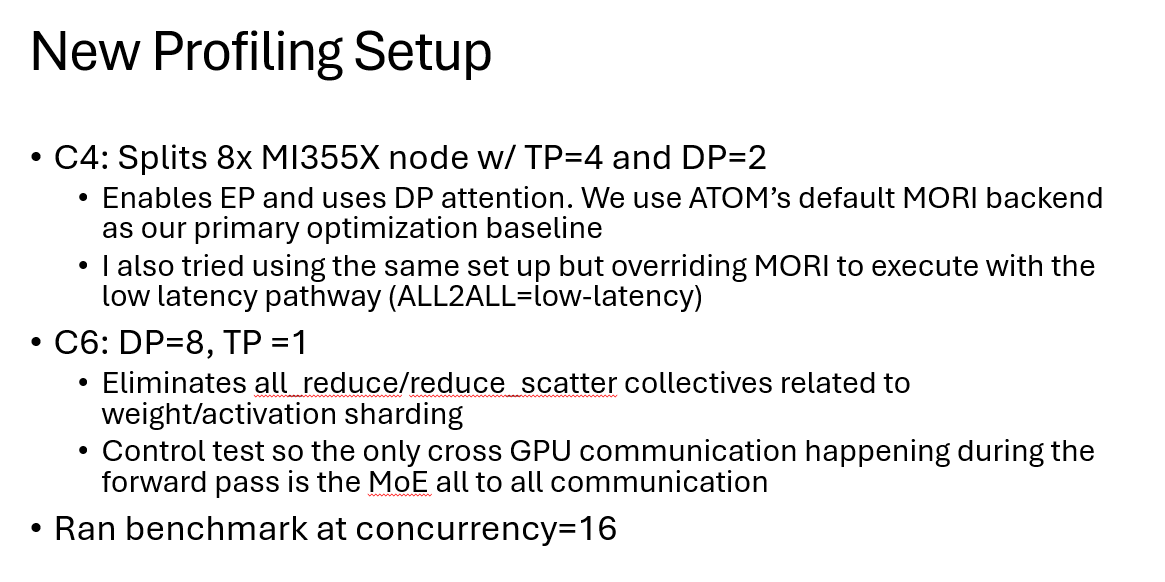
\includegraphics[width=\linewidth]{img/image004.png}
\end{column}
\begin{column}{0.46\textwidth}
\footnotesize
\begin{itemize}
  \item \empr{C4 = TP4 $\times$ DP2 + EP + DP-attention.} This is the real serving config; it is the \emph{only} mode where the MoE all-to-all (\mc{EpDispatch}/\mc{EpCombine}) fires --- it requires \mc{dp\_size>1} \emph{and} \mc{--enable-expert-parallel}. We use ATOM's default MORI backend as the \empy{primary baseline}, and also probed MORI's low-latency all2all path.
  \item \empr{C6 = DP8, TP1.} Control: removes the TP all-reduce/reduce-scatter entirely, so the \emph{only} cross-GPU traffic in the forward pass is the MoE all-to-all. Confirms the gather is an EP-flag artifact, not TP noise.
  \item Benchmarked at concurrency 16 (decode-heavy).
\end{itemize}
\end{column}
\end{columns}
\end{frame}

% ------------------------------------------------------------------
\begin{frame}{Step 0 --- profiling result: comm is 14--16\% of \emph{all} GPU time}
\begin{columns}
\begin{column}{0.46\textwidth}
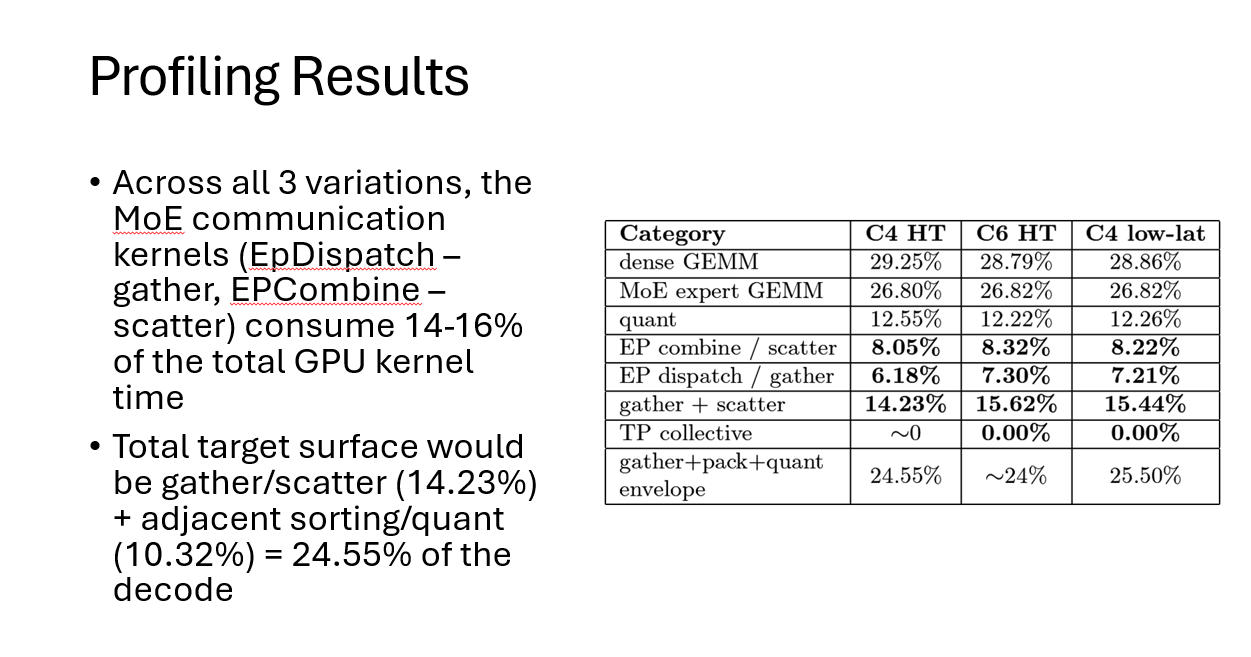
\includegraphics[width=\linewidth]{img/image001.png}
\end{column}
\begin{column}{0.52\textwidth}
\footnotesize
Stable across all three variants (C4 HT, C6 HT, C4 low-lat):
\begin{itemize}
  \item \empr{gather + scatter = 14--16\%} of total GPU kernel time (\mc{EpDispatch} $\sim$6--7\% + \mc{EpCombine} $\sim$8\%).
  \item Add the \emph{adjacent}, fusable sorting + quant ($\sim$10\%) $\Rightarrow$ a \empy{$\sim$24.5\% ``gather + pack + quant'' envelope} of the decode step.
  \item The expert GEMM itself is $\sim$27\%; dense (non-MoE) GEMM $\sim$29\%.
\end{itemize}
\examplebox{The target surface}{\footnotesize The fusable envelope --- everything \emph{around} the expert GEMM --- is a quarter of the decode step. That is what we attack.}
\end{column}
\end{columns}
\end{frame}

% ------------------------------------------------------------------
\begin{frame}{Why decode is a \emph{weight} wall --- and why that \emph{caps} the decode win}
\footnotesize
\empr{Key term: $M_e$ = rows (token--expert pairs) an expert processes.} At \empy{decode} you generate only a handful of tokens per step; with top-8 routing over 256 experts (32 local/GPU), even a 64-token step lands $\sim$16 rows on each local expert. Sweeping the stock region over batch size:
\begin{center}\scriptsize
\begin{tabular}{lrr}
\toprule
batch (tokens in flight) & rows/expert ($M_e$) & region $\mu$s \\
\midrule
\empr{decode} ($\sim$16 tokens) & 4   & 291.7 \\
decode ($\sim$64 tokens)        & 16  & 329.1 \\
mid ($\sim$256 tokens)          & 64  & 568.7 \\
\empy{prefill} ($\sim$1024 tokens) & 256 & 1416.7 \\
\bottomrule
\end{tabular}
\end{center}
\begin{itemize}\footnotesize
  \item \empr{The expert GEMM reads all 32 local experts' $\sim$1.4\,GB of fp8 weights from HBM \emph{every} step} --- a fixed $\sim$176\,$\mu$s floor (8\,TB/s), \emph{regardless of token count}. The region barely moves (292$\to$329) as tokens drop: it has hit that floor.
  \item \empr{Decode region $\approx$ 80\% weight floor $+$ 20\% boundaries} (gather/sort/quant/combine). That floor is \empy{identical} for us and the baseline (same fp8 weights), so fusion can't touch it $\Rightarrow$ \empr{even if every boundary were free, decode caps at $\sim$1.25$\times$} ($=1/0.8$); we land $\sim$1.03$\times$.
  \item \empr{Prefill has no such cap} --- its GEMM does token-scaled compute (not a fixed floor), so the \emph{whole} region is improvable $\to$ 1.56$\times$. \empy{(So ``shouldn't decode win more?'' --- no: a bigger boundary \emph{fraction} can't beat the weight wall that \emph{dominates} decode.)}
\end{itemize}
\end{frame}

% ------------------------------------------------------------------
\begin{frame}{The unfused baseline, drawn precisely}
\begin{columns}
\begin{column}{0.46\textwidth}
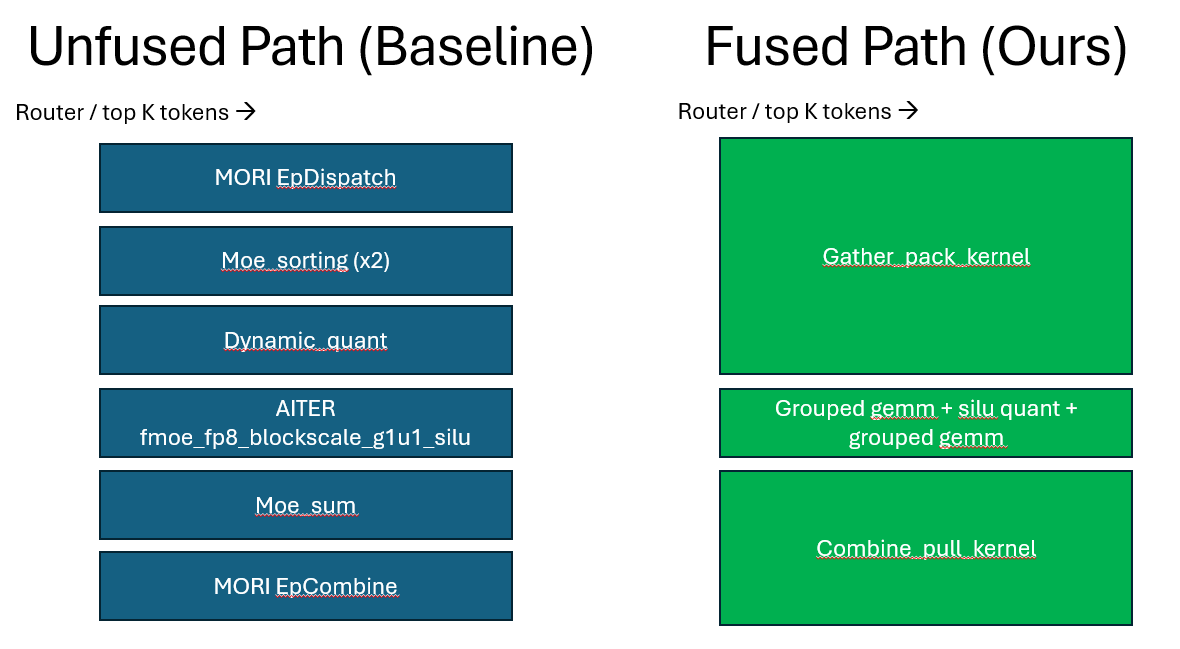
\includegraphics[width=\linewidth]{img/image003.png}
\end{column}
\begin{column}{0.52\textwidth}
\footnotesize
\mc{aiter.fused\_moe} is \emph{one Python call} but \emph{many GPU kernels}. The full C4-faithful region is \empr{seven stages}:
\begin{enumerate}\footnotesize
  \item MORI \mc{EpDispatch} \hfill (XGMI gather)
  \item \mc{moe\_sorting} pass 1 \hfill (counts/offsets)
  \item \mc{moe\_sorting} pass 2 \hfill (scatter to expert order)
  \item \mc{dynamic\_quant} \hfill (bf16 $\to$ fp8 + scales)
  \item \mc{fmoe\_..\_g1u1\_silu} \hfill (\empy{the good kernel}: fc1+SiLU+fc2)
  \item \mc{moe\_sum} \hfill (weighted top-k reduce)
  \item MORI \mc{EpCombine} \hfill (XGMI scatter)
\end{enumerate}
\examplebox{The inefficiency}{\footnotesize A \emph{good} expert kernel surrounded by \empr{expensive layout / materialization boundaries}.}
\end{column}
\end{columns}
\end{frame}

% ------------------------------------------------------------------
\begin{frame}{Why the unfused path bleeds: every boundary is an HBM round-trip}
\footnotesize
The expert kernel is \emph{not} the problem --- the stages \emph{around} it each read and re-write activations to HBM in a \emph{different} representation:
\begin{itemize}\footnotesize
  \item \empr{dispatch $\to$ sort:} tokens arrive in \emph{communication} order, but the GEMM needs \emph{expert-major} order. Sorting (2 passes) is pure layout traffic + sync --- \emph{not} GEMM work.
  \item \empr{sort $\to$ quant:} C4-faithful dispatch moves \emph{bf16} tokens; fp8 fmoe needs fp8+scales. \mc{dynamic\_quant} is a full read(bf16)/write(fp8) pass over the activation buffer.
  \item \empr{fmoe $\to$ combine:} fmoe writes expert outputs to HBM; \mc{moe\_sum}/\mc{EpCombine} read them back to accumulate weighted top-k and ship to origin ranks.
  \item \empr{launch/sync overhead:} most visible at \emph{decode} (tiny rows, fixed costs dominate).
\end{itemize}
\examplebox{Takeaway for the slide}{\footnotesize Unfused cost $=$ good expert kernel $+$ standalone \emph{sort} $+$ standalone \emph{quant} $+$ scatter \emph{combine}, each paying a real HBM read/write at the boundary. \empy{None of that is matmul.}}
\end{frame}

% ------------------------------------------------------------------
\begin{frame}[fragile]{What we actually built --- fuse the \emph{region}, not the math}
\footnotesize
\vspace{0.5ex}
\begin{columns}
\begin{column}{0.48\textwidth}
\empr{Unfused (7 stages):}
\begin{lstlisting}
EpDispatch
 -> moe_sorting x2
 -> dynamic_quant
 -> fmoe[fc1 + SiLU*up + fc2]
 -> moe_sum
 -> EpCombine
\end{lstlisting}
\end{column}
\begin{column}{0.48\textwidth}
\empy{Ours (region-fused):}
\begin{lstlisting}
gather_pack       [IRIS]
 -> grouped_b0 fc1  [HK]
 -> silu_quant      [HK]
 -> grouped_b0 fc2  [HK]
 -> combine_pull   [IRIS]
\end{lstlisting}
\end{column}
\end{columns}
\vspace{1ex}
\begin{itemize}\footnotesize
  \item \empy{[HK] HipKittens} does the on-GPU compute (fc1/fc2 GEMM, SiLU$+$requant, the local reduce); \empy{[IRIS]} does the cross-GPU communication (the gather pull, the combine write). \empr{No aiter} --- its \mc{fmoe} is the baseline we replace.
  \item This is the design from our meeting: \emph{HipKittens kernels for the math, an IRIS load/store on the MoE side for the comm.}
  \item \empr{We own the intermediate layouts}, so the comm \emph{produces} the GEMM's input layout --- killing the standalone sort, the quant pass, and the scatter combine.
\end{itemize}
\end{frame}

% ------------------------------------------------------------------
\begin{frame}{Kernel 1 --- \mc{gather\_pack} (IRIS): the communication \emph{is} the sort}
\footnotesize
Replaces MORI \mc{EpDispatch} $+$ the two \mc{moe\_sorting} passes. For each routed row we look up its source \mc{(rank,\,row)} from the routing metadata, then issue \empy{one IRIS \mc{ctx.load(ptr, src\_rank)}} --- a direct XGMI read of that row's 16 fp8 bytes $+$ its fp32 scale --- straight into our \emph{expert-major} packed buffer. Rows sourced from this same GPU skip XGMI (plain local load).
\begin{itemize}\footnotesize
  \item \empr{No sort pass:} the slot we write \emph{is} the expert-major row the GEMM wants --- communication and layout become one pass.
  \item \empr{``Zero sentinel'' $=$ a poison-free pad.} To run all 32 experts in one launch each expert's row-block is padded; padding/unrouted rows are written as fp8 \mc{0x00} with scale \mc{0}, so they multiply to \empy{exactly zero} in the GEMM --- a padded row can never corrupt a real expert's output.
  \item \empy{Comm/compute overlap, demonstrated (the meeting's goal).} In an overlap prototype we folded the fp8$\to$bf16 dequant \emph{into} this gather so it runs while the XGMI loads are still in flight: \empr{gather$+$dequant 162\,$\mu$s} vs \empr{gather-only 168\,$\mu$s} --- the dequant is \emph{hidden}, i.e.\ free. (The shipped region runs the dequant as a separate vectorized kernel; the harder \emph{in-GEMM} overlap is on the ``what didn't work'' slide.)
\end{itemize}
\end{frame}

% ------------------------------------------------------------------
\begin{frame}{Kernel 2 --- the expert GEMM \mc{grouped\_b0} (HipKittens)}
\footnotesize
The kernel that does the actual expert matmuls --- \emph{both} fc1 and fc2. It is our own HipKittens CDNA4 GEMM, not aiter:
\begin{itemize}\footnotesize
  \item \empy{8 waves, 256$\times$256$\times$64 tiles}, double-buffered shared$\to$register \emph{ping-pong}, \mc{mma\_ABt} (16$\times$16$\times$32 MFMA) into an fp32 accumulator --- written in HipKittens tile types (\mc{st\_bf} shared, \mc{rt\_bf} register, \mc{rt\_fl} accumulator).
  \item \empr{One thread-block per per-expert tile}, launched from a flat task list, so all 32 local experts compute in \emph{one} launch (this is what replaces aiter's grouped \mc{fmoe} GEMM).
  \item \empr{It consumes bf16.} The gather's packed A is fp8, so a \empy{vectorized dequant kernel} (\mc{fp8x4}$\to$\mc{bf16}, coalesced) converts it right before the GEMM --- the ``dequant preamble.'' Vectorizing it (scalar $\to$ packed) cut $\sim$117\,$\mu$s off fc1.
  \item We dequant to bf16 then MFMA, so \empy{the prefill GEMM is bf16-precision} --- that's where the clean RMS 0.018 comes from. (Decode swaps in a native-fp8 variant --- next slide.)
\end{itemize}
\end{frame}

% ------------------------------------------------------------------
\begin{frame}{Kernel 3 --- the activation \mc{silu\_quant} (HipKittens) --- \emph{not} a matmul}
\footnotesize
This is the \emph{middle} of the FFN, between fc1 and fc2: read fc1's output $C_1=$ gate$\|$up, compute $h=\mathrm{SiLU}(\text{gate})\cdot\text{up}$, then \empy{re-quantize $h$ to fp8} (per-128 block scale $=$ amax$/448$) so fc2 can consume it. No GEMM --- just activation $+$ requant.
\begin{itemize}\footnotesize
  \item \empr{Why a ``PyTorch'' baseline below, not the unfused path:} aiter does this activation \emph{inside} its monolithic \mc{fmoe}, so there is \emph{no} standalone unfused activation to race. When we split the region we had to write it ourselves --- and our first cut just called PyTorch's \mc{silu\_and\_quant}. The table is the optimization of \emph{our own} kernel:
\end{itemize}
\begin{center}\scriptsize
\begin{tabular}{lr}
\toprule
our v1 (calls PyTorch silu$+$quant) & 471\,$\mu$s \\
fused into one kernel & 127\,$\mu$s \\
\empy{+ local-amax (16-way vs 128-way atomics)} & \empr{38.6\,$\mu$s} \\
\bottomrule
\end{tabular}
\end{center}
\empr{The big jump (127$\to$38.6):} the per-128 amax was \emph{every} thread doing an \mc{atomicMax} into shared memory --- 128-way contention. Instead each thread keeps a \emph{local} amax over its own contiguous slice and does \emph{one} \mc{atomicMax} (16-way). (At decode a task-driven variant that skips padded rows reaches 7.2\,$\mu$s.)
\end{frame}

% ------------------------------------------------------------------
\begin{frame}{Kernel 4 --- \mc{combine} (IRIS): beating MORI's own combine}
\footnotesize
The combine is the \emph{reverse} of the gather --- send each expert-output (fc2) row back to its origin token, scaled by the route weight, summing the up-to-8 expert contributions per token.
\begin{itemize}\footnotesize
  \item \empr{v1 --- scatter.} One block owns one fc2 row; for each element it does an \empy{IRIS atomic-add (\mc{ctx.fetch\_add})} into the origin token's fp32 accumulator on the \emph{origin rank} over XGMI. The atomic is needed because top-8 means several expert outputs land on the same token. $\Rightarrow$ \empr{788\,$\mu$s}.
  \item \empr{Diagnosis --- the bytes, not the atomics.} Dropping the atomic saved $\sim$4\%; vectorizing the stores, 0\%. It is \empy{XGMI write-bandwidth bound}: $8192\times7168\times4$B $\approx$ \empy{234\,MB} of fp32 remote writes. The only lever is \emph{fewer bytes}.
  \item \empr{Fix --- pull / gather-reduce.} Invert it: each \emph{destination} token gathers its $\leq$8 fc2 rows from the \emph{local} buffer, sums them in fp32 locally (\empy{no cross-rank atomics}), and writes \emph{one bf16} row home via \mc{ctx.store} (234$\to$117\,MB). The local fp32 sum is what makes a bf16 result correct under collisions.
\end{itemize}
\vspace{-0.5ex}
\begin{center}\scriptsize
\begin{tabular}{lr}
pull, bf16, cells \emph{sorted} by dst\_rank & 934\,$\mu$s \;(\emph{worse!}) \\
\empy{pull, bf16, cells \emph{round-robin'd} across dst\_rank} & \empr{386\,$\mu$s} \\
MORI \mc{EpCombine} (the baseline) & 398\,$\mu$s \\
\end{tabular}
\end{center}
\empr{Decisive:} sorting destinations hammers one XGMI link at a time; \empy{round-robin spreads concurrent blocks over all 8 links} --- same bytes, 2.4$\times$ faster, below MORI.
\end{frame}

% ------------------------------------------------------------------
\begin{frame}{The decode GEMM --- a \emph{different}, skinny BM=16 native-fp8 kernel}
\footnotesize
\empr{Decode swaps in a different GEMM than prefill.} Prefill's \mc{grouped\_b0} uses 256-row tiles; at decode each expert has only $\sim$4--16 real rows, so a 256-row tile is $\sim$94\% padding and the GEMM goes \emph{compute-bound grinding zeros}. \mc{grouped\_b0\_gemm\_decode} uses a \empy{skinny BM=16 tile} (the MFMA's minimum M) --- that drops the padded compute \emph{below} the weight-stream floor, so decode finally becomes weight-memory-bound, where the one lever is \empy{fp8 weights} (half the HBM bytes).
\begin{itemize}\footnotesize
  \item \empr{Native fp8 with no fp8 load path:} HipKittens can't load fp8 to registers, so we \empy{store fp8 but \emph{load as} a half-width bf16 tile} (the fast path), unpack fp8$\to$bf16 in-register, bf16$\times$bf16 MFMA --- weights \emph{pre-swizzled offline} into fragment order. Standalone: \empy{3.97\,TB/s, 1.46$\times$ over bf16}, RMS 0.0037 --- matches aiter's fused fp8 (decode 171.0 vs 171.6 TFLOP/s).
  \item \empr{A subtle bug (14 experiments):} a stable wrong answer (RMS $\approx$ 0.71) $+$ an apparent hang. \empy{Not a data bug --- a compiler scheduling hazard}: the async \mc{ds\_read}'s inline-asm output looked register-ready, so the compiler hoisted the first \mc{mma} \emph{above} the \mc{s\_waitcnt} that waits for the data $\Rightarrow$ it multiplied not-yet-arrived operands (garbage $=$ 1/$\sqrt2$); the bad read also computed out-of-bounds addresses $=$ the ``hang.''
  \item \empr{Fix:} a one-line scheduling barrier (\mc{s\_waitcnt lgkmcnt(0)} $+$ \mc{sched\_barrier}) before the mma --- both symptoms gone.
\end{itemize}
\end{frame}

% ------------------------------------------------------------------
\begin{frame}{How we benchmarked (the part experts will poke at)}
\footnotesize
\empr{Compare regions, not kernels --- define the region by its I/O boundary} (enter: routed bf16 tokens + top-k; exit: combined bf16 outputs, token order) and measure \emph{both} sides over it.
\begin{itemize}\footnotesize
  \item \empy{Same node, same operating point.} Nodes vary $\sim$1.8$\times$ in speed across the cluster --- an early ``decode 920\,$\mu$s loss'' was just a throttled node (its prefill was 2198 vs 1240). \empr{Always run $b_1$ and $b_3$ back-to-back on one node.}
  \item \empy{Pre-warm aiter.} aiter JIT-compiles its fmoe per (shape,dtype) into a \emph{container-local} cache ($\sim$10\,min cold) --- a ``hang'' that is really a cold cache. Warm it before timing.
  \item \empy{MAX over 8 ranks}, device-event timed, warmup + median, \empr{correctness gate (RMS) before timing}, reported at \emph{decode and prefill}.
  \item Baseline $=$ stock MORI \mc{EpDispatch} (bf16) $+$ aiter \mc{fused\_moe} $+$ MORI \mc{EpCombine} --- the C4-faithful production chain.
\end{itemize}
\end{frame}

% ------------------------------------------------------------------
\begin{frame}{Result --- PREFILL: 1.56$\times$ (the strong, clean claim)}
\footnotesize
8 full MI355X, same node (thor-4), correctness-gated:
\begin{center}
\begin{tabular}{lrrr}
\toprule
region & fused $b_1$ & unfused $b_3$ & speedup \\
\midrule
\empy{prefill (TOTAL\_M=8192)} & \empr{1247\,$\mu$s} & 1941\,$\mu$s & \empr{1.56$\times$} \\
\bottomrule
\end{tabular}
\end{center}
Per-stage decomposition (illustrative; \emph{don't mix denominators across nodes}):
\begin{center}\footnotesize
\begin{tabular}{lrr}
\toprule
stage & unfused & fused (ours) \\
\midrule
dispatch / gather   & 290 & \empy{147} \\
expert FFN GEMM     & 2622 (fmoe) & 921 (fc1) + 481 (fc2) \\
activation          & --- (in fmoe) & \empy{39} \\
combine             & 398 (MORI) & \empy{387} (pull) \\
\midrule
\textbf{region}     & \textbf{3246} & \textbf{1974} \;($1.64\times$) \\
\bottomrule
\end{tabular}
\end{center}
\empr{Why prefill wins:} the GEMM is bandwidth/compute-rich, so the eliminated boundaries (sort, quant materialization, scatter combine) are pure savings --- \emph{and} our combine beats MORI, our act is near-free, and the dequant hides under the gather. \empy{Bonus: our prefill GEMM is bf16-dequant ($\to$ RMS 0.018), \emph{higher} precision than aiter's fp8.}
\end{frame}

% ------------------------------------------------------------------
\begin{frame}{Result --- DECODE: honest, marginal, and \emph{why}}
\footnotesize
Same node (thor-4), warm aiter, correctness-gated:
\begin{center}
\begin{tabular}{lrrr}
\toprule
region & fused $b_1$ & unfused $b_3$ & verdict \\
\midrule
\empy{decode (TOTAL\_M=512)} & \empr{516.5\,$\mu$s} & 527\,$\mu$s\;(533 canon.) & $\sim$2--3\% win \\
\bottomrule
\end{tabular}
\end{center}
Per-stage: gather 41.5 $+$ fc1 274 $+$ \empy{act 7.2} $+$ fc2 150 $+$ combine 47.
\begin{itemize}\footnotesize
  \item \empr{Why only $\sim$2--3\%:} as the cost model predicted, decode is \empy{weight-bound} --- fc1$+$fc2 $=$ 424 of 516\,$\mu$s is just the two fp8 weight streams near the in-region HBM rate. The boundaries we removed were only $\sim$18\% to begin with; we recovered the act tax (25$\to$7\,$\mu$s) and edged ahead.
  \item \empr{The RMS caveat (be precise).} The fp8-weight region scores RMS 0.057 vs a bf16-weight reference; bf16 weights would score 0.018. That 0.018$\to$0.057 jump \emph{is} e4m3's $\sim$3.6\% per-weight error (scale-invariant; finer scales don't help). \empy{But the aiter baseline \emph{also} runs fp8 weights} (\mc{fmoe\_bf16\_blockscaleFp8}) --- so 0.057 is production's \emph{own} precision class. A strict RMS$<$0.05 needs bf16 on a matmul $=$ $+135\,\mu$s $=$ a decode \emph{loss}. It's a real $\mu$s-vs-precision tradeoff, and at \emph{matched} precision decode wins.
\end{itemize}
\end{frame}

% ------------------------------------------------------------------
\begin{frame}{What didn't work (1/2) --- and the architectural reason}
\footnotesize
\begin{itemize}\footnotesize
  \item \empr{Host-stream overlap (gather $\|$ GEMM on two HIP streams).} Even after fixing chunked-gather grid collapse, concurrent $=$ $-12$ to $-153\,\mu$s vs serial. \empy{Reason:} the B0 GEMM already saturates the CUs, so two streams just time-slice. The expert GEMM is not idle enough to hide the gather at the \emph{stream} level.
  \item \empr{In-kernel gather-under-MFMA (the ``V2'' dream).} The only existing body that does remote gather under MFMA runs \empy{35.8 vs 466 TFLOP/s --- 13$\times$ slower}. \empy{Reason:} the fast B0 body has \emph{no} producer/consumer warp split and \emph{no} A-reuse across N-subtiles; blocking remote loads stall the waves instead of hiding comm. This needs a \emph{different} GEMM body (async A-fill + reuse), not a patch --- a real open direction.
\end{itemize}
\examplebox{The honest thesis boundary}{\footnotesize Comm/compute overlap \emph{works} where compute sits in comm's shadow (the dequant-in-gather). It does \emph{not} work as warp-level gather-under-MFMA on today's peak GEMM body --- the GEMM is too busy and not structured for it.}
\end{frame}

% ------------------------------------------------------------------
\begin{frame}{What didn't work (2/2)}
\footnotesize
\begin{itemize}\footnotesize
  \item \empr{Native fp8 at BM=256.} $+8$\% at full occupancy, neutral/negative at decode. \empy{Reason:} at BM=256, decode is \emph{compute-bound on padding}, so halving weight bytes doesn't help. fp8 only pays off once a small-BM tile makes decode weight-\emph{memory}-bound.
  \item \empr{Register double-buffer for the decode tile.} $\sim$3$\times$ \emph{slower}. \empy{Reason:} doubling the A/B register tiles blew VGPR $\to$ occupancy collapse below \mc{launch\_bounds}; at BM=16, latency hiding $=$ \emph{occupancy} (many warps), not a wider per-thread pipe. LDS double-buffering (VGPR-cheap) was the right tool.
  \item \empr{Compacting the GEMM padding (Mpacked 8192$\to$512).} Reassessed as \emph{high-risk / low-reward}: the weight stream is a \emph{contiguous} per-expert buffer, so the padding adds compute that largely hides under it; the recoverable cost was the \emph{act} tax (already taken, 25$\to$7\,$\mu$s). Compaction would also break the ERB\,\%\,256 alignment the gather/GEMM rely on (history: rewrites $\to$ RMS$\approx$1.0). \empy{Profile before you pay.}
  \item \empr{Strict RMS$<$0.05 decode win.} Fundamental: it requires a bf16 matmul $=$ +135\,$\mu$s $=$ a loss. Not a bug to fix --- a precision floor to state honestly.
\end{itemize}
\end{frame}

% ------------------------------------------------------------------
\begin{frame}{Aside --- the ``padding tax,'' and is the comparison fair?}
\footnotesize
A natural expert question: \emph{why does our grouped GEMM pad each expert to 256 rows (8192 packed for $\sim$512 real at decode)?}
\begin{itemize}\footnotesize
  \item \empr{Why we pad:} flattening 32 experts into one launch requires each expert's region rounded up to the tile height (BM), so a tile never straddles two experts (the ``no-contamination'' invariant). Our 8-wave body uses BM=256.
  \item \empr{Does production have it too? Yes.} aiter's \mc{moe\_sorting} pads each expert to its tile granularity (\mc{block\_m} $\sim$16--32). \empy{Padding is inherent to grouped/sorted MoE GEMM} --- ours is just $\sim$8$\times$ coarser, a self-inflicted (fixable) handicap, \emph{not} an unfair benchmark.
  \item \empr{Does it cost wall-clock? Mostly no (we measured).} Because decode is weight-bound, the padding adds \emph{compute} that hides under the weight stream --- the one exposed cost was the \emph{activation} kernel launching one block per padded row, which we fixed (act 25$\to$7\,$\mu$s). The GEMM-side compaction wasn't worth the alignment risk.
\end{itemize}
\end{frame}

% ------------------------------------------------------------------
\begin{frame}{Summary --- aiter fuses the math; we fuse the region}
\footnotesize
\begin{columns}
\begin{column}{0.5\textwidth}
\empr{What the fusion buys (all measured, 8 full MI355X, pushed to GitHub):}
\begin{itemize}\footnotesize
  \item \empy{Prefill 1.56$\times$} over the production MORI+aiter chain --- the headline.
  \item A pull-combine \empy{below MORI's own} EpCombine (386 vs 398\,$\mu$s).
  \item Near-free activation (471$\to$7--39\,$\mu$s) and \empy{dequant hidden under the XGMI gather} (comm/compute overlap, demonstrated).
  \item Decode brought from a loss to a \empy{marginal win at production-matched fp8 precision}.
\end{itemize}
\end{column}
\begin{column}{0.5\textwidth}
\empr{The honest boundaries:}
\begin{itemize}\footnotesize
  \item Decode is a \emph{weight} wall --- fusion's ceiling there is $\sim$1.1--1.4$\times$, and the fp8 RMS floor is real.
  \item Warp-level gather-under-MFMA needs a new GEMM body (open work).
  \item Bigger decode levers are orthogonal: more EP shards, fp4 weights, larger batch.
\end{itemize}
\vspace{1ex}
\empr{Substrate:} HipKittens (CDNA4 8-wave MFMA, fp8/bf16 tiles, \mc{sched\_barrier}) + IRIS (XGMI \mc{ctx.load}).
\end{column}
\end{columns}
\vspace{0.5ex}
\examplebox{One line}{\footnotesize Make the communication produce the compute layout, hide the conversions in its shadow, and reduce on \emph{pull} not scatter --- and the fused expert region beats the unfused production baseline, decisively at prefill.}
\end{frame}

% ------------------------------------------------------------------
\begin{frame}{Backup --- numbers at a glance}
\scriptsize
\begin{tabular}{lrr}
\toprule
quantity & ours & baseline \\
\midrule
prefill region (8192) & 1247\,$\mu$s & 1941\,$\mu$s \;($1.56\times$) \\
decode region (512), warm same-node & 516.5\,$\mu$s & 527\,$\mu$s \\
combine & 386\,$\mu$s (pull) & 398\,$\mu$s (MORI) \\
activation & 38.6 / 7.2\,$\mu$s & --- (inside fmoe) \\
dequant (folded in gather) & $\approx$0 (162 vs 168 gather-only) & full pass \\
decode GEMM (standalone) & 3.97\,TB/s, 1.46$\times$ over bf16, RMS 0.0037 & aiter parity \\
prefill RMS / decode RMS & 0.018 / 0.057 & (fp8 class) \\
\midrule
scatter combine (rejected) & 788\,$\mu$s (write-BW-bound, 234\,MB) & \\
in-kernel gather-under-MFMA (rejected) & 35.8 vs 466 TFLOP/s & \\
host-stream overlap (rejected) & $-12$ to $-153\,\mu$s & \\
\bottomrule
\end{tabular}
\vspace{1ex}

\scriptsize Repo: \mc{github.com/subha-amd/iris} (branch \mc{subha/moe-dispatch-v0}). Decode is weight-bound; gather/combine $=$ $\sim$18\% of the decode region, $\sim$14--16\% of total GPU time.
\end{frame}

\end{document}
